\documentclass[10pt,letterpaper]{article}
\usepackage{geometry}
\geometry{margin=1in}
\usepackage{graphicx}
\usepackage{tikz}
\usepackage{float}
\usepackage[style=numeric,backend=biber]{biblatex}

\addbibresource{Lab_2.bib}
\setlength{\parindent}{0pt}
\setlength{\parskip}{0.5em}

%make lists tighter
\usepackage{enumitem}
\setlist{nolistsep}

%reduce spacing before and after section
\usepackage{titlesec}
% reduce section, subsection, etc spacing
\usepackage{titlesec}
\titlespacing*{\section}{0pt}{0\baselineskip}{0\baselineskip}
\titlespacing*{\subsection}{0pt}{0\baselineskip}{0\baselineskip}
\titlespacing*{\subsubsection}{0pt}{0\baselineskip}{0\baselineskip}

%reduce list spacing
\usepackage{enumitem}
\setlist{nosep}

\usepackage[hidelinks]{hyperref}

\title{Lab 2 - Linguistics Data, Stat 215A, Fall 2025\vspace{-2em}}

% submission must not contain your name
% but feel free to make a version for yourself with your name on it
% \author{Your name}


\begin{document}



\maketitle


\section{Introduction}\label{introduction}

Linguistics was originally considered a qualitative field. Before the advent of modern technologies such as fMRI, sagittal imaging, and even recently electromagnetic articulography, linguistics relied on qualitative data collected by field analysts. Phoneticist relied on traditional ``by ear" methods of transcription. Studies in archaeological linguistics, orthography, and semantics were qualitative endeavors, relying solely on the domain expertise of linguists. However, thanks in part to democratization of computing, linguists begin to collect larger and larger qualitative data sets bring about the advent of linguistic computing.One of the first linguistic fields to make this transition is dialectology (the study of dialects). Nerbonne and Kretzschmar call attention to the dialetometery (the measure of the difference between different dialects\cite{nerbonne_introducing_2003}). In order to take into account the complex dynamics of linguistic and geographical variations there arose a need for ``computation techniques" \cite{nerbonne_introducing_2003}. This work quickly progressed to ``the analysis of complex variation data" from which modern linguistics as a highly technical and computation field has emerged \cite{nerbonne_progress_2006}.

The purpose of this paper is to undertake a similar dialectromic analysis of dialect data for the United States as collect by the Harvard Dialect Survey. Focusing on lexographic data, we employ dimension reduction techniques, Principal Components Analysis and t-SNE to visualize important lexographic features in the American dialect. We discuss the advantages and disadvantages of both approaches rooted in the context of linguistic survey data. We then employ K-Means Clustering to try to identify dialect groups and compare them to know geographical groups. We contrast these results with an agglomerative clustering approach through two linkage parameters--ward and average. Throughout this analysis, we employ the PCS frame work to analyze stability and document decisions in the analysis pipeline and their downstream impacts\cite{yu2024veridical}. In doing so, we gain understanding about both the uncertainty in the data science pipeline, as well as understanding the variability of the data. 

\section{The Data}\label{data}



This analysis uses the data from the Harvard Dialect Survey conducted by Prof. Bert Vaux. The dialect survey is an online survey that uses a series of questions spanning phonetic and lexical features of American English. Questions include questions like ``Do you cut or mow the lawn?" or ``What do you call the box you bury a dead person in?" Everyone who takes the survey answers these questions as well as self reporting their location as their state and city. Latitude and longitude were then imputed by based on the centroid of the reported city. This imputation was completed beforehand but outside sources. This location information provides the basis for the interpretation of the clustering explored in \ref{clustering}. In total, the data consists of 47,471 respondents answering 121 questions plus demographic information from around 2000-2005\footnote{The exact dates are a bit hazy. There were a couple of releases of the survey and it is unclear if the data spans the entirety of the survey. We are fairly certain that data from the 1997-99 handout version is not included.}.\\ 

While there are questions concerning phonetics, we are only concerned with the lexical questions. In particular we will look at two questions that revolve around common items used commonly across the United States: shoes and drinking fountains (see \ref{data-exploration}). The lexical data will allow us to understand measures of dialect similarity by understanding how different people use different lexicons in different geographic locations to try to categorize dialect groups. 


It is important to note that this data was collected as a public survey which was open to anyone until the completion of the survey. As such, we are cognizant about the limitations of the data. There is inherent response bias as is common with surveys. Moreover, there was no way for linguist to verify the the data collected. There was no professional field linguist ensure supervising every participant's response to the survey. These are limitations that cannot be accounted for--and should not be accounted for--in the data analysis.

\subsection{Data Cleaning}\label{data-cleaning}

The cleaning procedure used on this data are relatively minimal as there is not much ability to reason through missing data and to impute. That being said, since this data was collected as a survey and not in a controlled setting there were a few issues that had to be addressed. The first major issue is that not everyone who took the survey answered every question. All missing values were assigned a 0 (the answer choices ``a", ``b", ``c" are enumerated ``1", ``2", ``3" in the original data set). We change all 0's given as answers to ``NaN" to not confuse analysis.\\

The other most glaring issue is most certainly due to the public and unsupervised nature of the survey. The location data is incomplete. Which surprisingly well populated, there are just over a thousand observations with missing location data, either city, state, zip code, or latitude and longitude. Since we want to ensure that the analysis is conducted consistently using data from the United States (as even a fraction of respondents from other countries could impose massive outliers), we remove all those observations that do not have a self reported state or a state that is outside of the United States. Closer inspection of the states reveals a variety of Canadian provinces and abject gibberish. Trying to impute based on the state is not reasonable. We find this decision to be sensible and believe that the downstream impacts are negligible.\\

We use this minimally processed version of the data for EDA as outlined in the next section. However, for the dimension reduction and clustering carried out in Sections \ref{dimension-reduction} and \ref{clustering} we include a few more prepossessing steps. 

\subsubsection{Reprocessing}

% We first create a new variable in the location data which we call ``Region". The region is broken down into nine different geographical regions based on colloquial regional categorizations of states (Table \ref{tab:region_map}). 

% \begin{table}[ht]
% \centering
% \caption{Regional Classification of U.S. States}
% \label{tab:region_map}
% \begin{tabular}{ll}
% \hline
% \textbf{Region} & \textbf{States} \\
% \hline
% West Coast & CA, OR, WA \\
% Mountain & AZ, CO, ID, MT, NV, NM, UT, WY \\
% Southwest & TX, OK, AR, LA \\
% South & AL, FL, GA, KY, MS, NC, SC, TN, VA, WV \\
% Midwest & IL, IN, IA, KS, MI, MN, MO, NE, ND, OH, SD, WI \\
% East Coast & DE, MD, NJ, NY, PA \\
% New England & CT, ME, MA, NH, RI, VT \\
% Alaska & AK \\
% Hawaii & HI \\
% \hline
% \end{tabular}
% \end{table}
% This mapping provides a less granular view of the location data which is useful in data visualization after dimension reduction (Section \ref{dimension-reduction}). These labels are not used in any of the modeling other than for use as a convenient label. \\

In order to capture the different answers for each question, each of which has a different number of possible responses, we do binary encoding the data frame. This leaves a sparse data frame with individual level data; however we want to understand larger region variations beyond a person to person basis. To counter this issue, we bin the lat by rounding the latitude and longitude top the nearest degree. Since the latitude and longitude were imputed based on the city, we do not feel that we are losing information as this was already a ``best guess". Finally, we divide the responses in each bin by the total number of respondents in the bin. This helps ensure that we do not favor population centers do to a difference in magnitude. While it seems unlikely that we can fully avoid the issue of the population density, this is a step to help mitigate the impact in the clustering process.

\begin{figure}
    \centering
    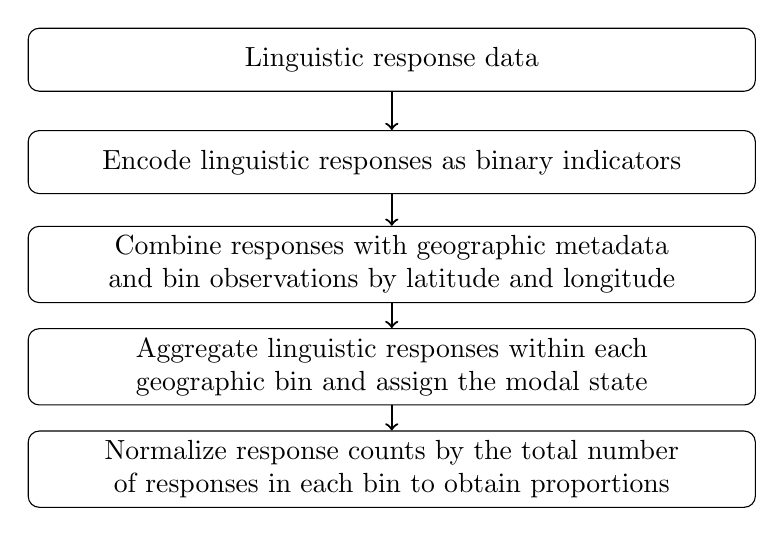
\begin{tikzpicture}[
    node distance=1.3cm,
    every node/.style={
        draw,
        rounded corners,
        align=center,
        text width=9cm,
        minimum height=0.8cm
    },
    arrow/.style={->, thick}
]

\node (start) {Linguistic response data};

\node (encode) [below of=start]
    {Encode linguistic responses as binary indicators };

\node (geo) [below of=encode]
    {Combine responses with geographic metadata and bin observations by latitude and longitude};

\node (aggregate) [below of=geo]
    {Aggregate linguistic responses within each geographic bin and assign the modal state};

\node (normalize) [below of=aggregate]
    {Normalize response counts by the total number of responses in each bin to obtain proportions};

\draw [arrow] (start) -- (encode);
\draw [arrow] (encode) -- (geo);
\draw [arrow] (geo) -- (aggregate);
\draw [arrow] (aggregate) -- (normalize);

\end{tikzpicture}
    \caption{Preprocessing Workflow}
    \label{fig:preprocessing}
\end{figure}

\subsection{Exploratory Data Analysis}\label{data-exploration}
To begin exploratory data analysis we select two questions from the dialect survey. To try to maintain a consistent narrative, we select two questions that are both differences in the name of a common, everyday object. We chose question $73$: ``What is your *general* term for the rubber-soled shoes worn in gym class, for athletic activities, etc.?" and question $103$: ``What do you call the thing from which you might drink water in a school?"\\

First, looking at question $73$ we find a large array of responses including shoes, sneakers, gym shoes, etc. We take the three most popular responses ``sneakers", ``tennis shoes", and ``gym shoes". We visualize this in Figure \ref{fig:shoes_map}. The answer ``gymshoes" is clearly far less popular. Focusing on the ``sneakers" vs ``tennis shoes" dichotomy we can see a clear distinction in the new England region with a larger concentration of people who prefer ``sneakers". Conversely people in the the Midwest tend to prefer ``tennis shoes". Beyond this 

\begin{figure}[H]
    \centering
    \includegraphics[width=1\linewidth]{shoes_map.png}
    \caption{Map of responses to terms used for gym shoes with top three answers represented.}
    \label{fig:shoes_map}
\end{figure}

distinction, the sparsity on the middle of the country makes it difficult to postulate any further. Moreover, we can clearly see the population hubs are expressed on the map. We must be careful to not extrapolate from that information. \\

Similarly, we consider the question about what one calls the thing from which you drink water. We visualize in Figure \ref{fig:water_fountin_map} where we can observe a concerntration of the use of ``drinking fountain" in the great lakes region and on the west coast. ``Water fountain" is certainly in favor with those along the east coast. We find a small cluster of folks in Wisconsin who prefer the far more whimsical ``bubbler". Again, the sparsity of responses in the middle of the country does make interpretation more difficult. 
\begin{figure}[H]
    \centering
    \includegraphics[width=0.75\linewidth]{water_fountain_map.png}
    \caption{Map of response to terms used to describe thing from which one might drink at school with top three answers displayed.}
    \label{fig:water_fountin_map}
\end{figure}

Using this insights, we consider how the combination of these observations might provide a better look at potential dialect regions. To answer this question, we consider the correlation between the top two most common answers to both of the aforementioned questions. In Figure \ref{fig:heatmap} we present a heat map of the relative frequencies of the top two most popular answers to questions considered in Figures \ref{fig:shoes_map} and \ref{fig:water_fountin_map}. We find the most common combination of answers is ``tennis shoes" and ``water fountain" followed closely by ``sneakers" and ``water fountain". The combination of ``tennis shoes" and ``drinking fountain" also has a significant percentage.

\begin{figure}[H]
    \centering
    \includegraphics[width=0.8\linewidth]{heatmap_correlation_Q103_Q073.png}
    \caption{Heatmap displaying the relative frequencies of answers to preferred term for drinking apparatus and shoes worn for physical activity.}
    \label{fig:heatmap}
\end{figure}

We then want to see if these observed combinations express themselves on a map as visualized in \ref{fig:comb_map}. We still see that New England and the great lakes region are expressed in this graph with the American south expressing similar dialect choices. Moving towards the west, it becomes difficult to parse the map as the population clusters are sparsely distributed and densely packed. 

\begin{figure}[H]
    \centering
    \includegraphics[width=0.8\linewidth]{comb_map.png}
    \caption{Map of combined answers.}
    \label{fig:comb_map}
\end{figure}
To help combat the issue of the sparsity, we take the majority combined answer in each state to define that states dialect as visualized in Figure \ref{fig:combin_bystate}. 
\begin{figure}[H]
    \centering
    \includegraphics[width=.75\linewidth]{newplot.png}
    \caption{Dominant combination of answers by State}
    \label{fig:combin_bystate}
\end{figure}
We find that the combination of ``drinking fountain" and ``sneakers" is not dominant in any of the states. We clearly see the New England and northern Atlantic coast area defined on the map. Surprisingly, we find Florida and Hawaii have the same dominant combination which suggests a linguistic connect between the two areas. We similarly see the south grouped together as we would expect with the addition of parts of the Midwest. The delineation between East and West is also strongly suggested. It is unclear is this is a factor of the sparsity or it represents a possible trend. Using these preliminary results we can postulate a three way partition of states. 
\section{Dimension Reduction}\label{dimension-reduction}
For dimension reduction we provide two common dimension reduction techniques: Principal Components Analysis (PCA) and t-SNE (t-Distributed Stochastic Neighbor Embedding). Since t-SNE takes in principal components for projection we first discuss the PCA.

\subsection{PCA}
Given the common scale of the data, as well as the strictly positive nature of the data even after reprocessing, we call into question the standardization steps taken in most PCA computations. As a result, we use Singular Value Decomposition (SVD) to reduce the dimensionality of the resulting geographic response matrix. SVD is closely related to PCA, but it gives us greater flexibility in deciding whether centering the data is appropriate for this application.
Standard PCA is typically performed after centering each feature by subtracting its mean. This transformation is useful when the goal is to study variation around the average observation. Here, however, the entries of our matrix are geographic response counts. The magnitude of these counts has a natural interpretation: it reflects the number of respondents in a geographic bin who selected a particular answer. Automatically centering each response variable would remove its overall mean and therefore change the interpretation of the geographic response patterns we are trying to capture.\\

\begin{figure}[H]
    \centering
    \includegraphics[width=1\linewidth]{svd_vs_pca_explained_variance.png}
    \caption{Explained Variance by components PCA vs SVD}
    \label{fig:skree}
\end{figure}

In Figure \ref{fig:skree} we present the explained variance by component for both SVD and PCA. As we expected, we find that SVD explains much more of the variance with the first few components, with the first component account for over $40\%$ of the variability in the data. For both SVD and PCA the change in explained cumulative variance is concerning as the change is very slow following the first component. This seems to suggest there is one set of features that has the biggest impact on the dialect separation in the United States. \\

Using the PCA and SVD scores, we can project the reduced-dimensional representations back onto the geographic map to examine how the dominant sources of variation are distributed spatially. In Figure \ref{fig}, we plot the geographic distributions of the first two SVD components. First, we note that the one-degree latitude by one-degree longitude binning performed during preprocessing produces the visible grid-like structure in the maps. This pattern is an artifact of the preprocessing procedure rather than a feature of the underlying dialect variation.

\begin{figure}[H]
    \centering
    \includegraphics[width=1\linewidth]{svd_geographic_distribution.png}
    \caption{SVD reduction visualized on map}
    \label{fig:svd_graph_dist}
\end{figure}

The first two components reveal a broad east--west pattern in the lexical response data, with the largest differences concentrated in the Rocky Mountain and southwestern regions. Thus, the dominant directions of variation identified by SVD are not geographically random; they correspond to substantial regional differences in lexical response patterns. However, these components do not reproduce several of the more localized geographic patterns observed during EDA. This suggests that the strongest sources of variation in the full response matrix capture broad regional differences, while finer-scale dialect structure is distributed across additional components. Consequently, the first two components provide evidence of broad geographic structure in the lexical data, but they are insufficient to fully characterize the spatial variation observed in the survey.  





\subsection{t-SNE}

After reducing the dimensionality of the geographic response matrix using SVD, we use $t$-distributed Stochastic Neighbor Embedding (t-SNE) as a nonlinear visualization method. t-SNE is a reasonable choice because the relationship among lexical response patterns need not be well represented by a linear low-dimensional subspace. We apply t-SNE to the low-dimensional SVD representation rather than directly to the full response matrix. This provides a computationally simpler representation while retaining the dominant variation identified by SVD. The resulting two-dimensional embedding provides an exploratory representation of the relationships among geographic bins. Rather than viewing the dimension reduction only in the abstract t-SNE space, we use the two resulting coordinates, $\mathrm{tSNE}_1$ and $\mathrm{tSNE}_2$, as attributes of each geographic bin and map them back onto their original geographic locations (Figure \ref{fig:tsne_map}). This allows us to examine whether patterns in the reduced response space exhibit meaningful geographic structure.

\begin{figure}[H]
    \centering
    \includegraphics[width=1\linewidth]{tsne_geographic_distribution.png}
    \caption{Geographic distribution of t-SNE scores for t-SNE1 and t-SNE2.}
    \label{fig:tsne_map}
\end{figure}

The map for $\mathrm{tSNE}_2$ reflects some of the structure uncovered in EDA. In particular, we see the emergence of the great lakes region as a group. However, there are several limitations to this approach that hamper interpretation. Most importantly, t-SNE is designed to preserve local neighborhoods rather than global distances, so the numerical values of $\mathrm{tSNE}_1$ and $\mathrm{tSNE}_2$ do not have a direct interpretation, and distances between geographic bins in the t-SNE space should not be interpreted as quantitative measures of dialect similarity. The method is also stochastic and sensitive to tuning parameters such as perplexity and random initialization, meaning that the precise embedding may change across runs. We used general hyperparameter and neglected tuning as there is no advantage to cluster on t-SNE. In addition, because t-SNE does not use latitude or longitude when constructing the embedding, geographic proximity is not explicitly incorporated into the dimension reduction. Thus, mapping the t-SNE coordinates geographically is useful for identifying spatial patterns in lexical similarity, but apparent geographic clusters should be viewed as exploratory rather than as definitive evidence of distinct dialect regions.

\section{Clustering}\label{clustering}
To further investigate structure in the reduced-dimensional data, we use both $k$-means and agglomerative hierarchical clustering. We are interested in determining whether geographic bins can be grouped according to similarities in their lexical response profiles, without imposing predefined dialect regions. We perform clustering on the SVD scores, allowing the clustering methods to operate on the dominant dimensions of variation rather than on the full, highly dimensional response matrix.
We use $k$-means for the simple and interpretable partitioning of the observations into groups. The method assigns each observation to the cluster with the nearest centroid, producing groups whose observations have similar SVD representations. This makes $k$-means particularly useful for examining whether the dominant variation identified by SVD corresponds to relatively distinct groups of dialect profiles. Pursuant to the preliminary results discussed in EDA, we try a $k$-means using $3$ centroids (Figure \ref{fig:k_means_3}).

\begin{figure}[H]
    \centering
    \includegraphics[width=0.7\linewidth]{kmeans_clusters_map.png}
    \caption{K-means clustering results for $k=3$}
    \label{fig:k_means_3}
\end{figure}

The $k$-means clustering appears to recover the broad east--west differences identified in the SVD maps, suggesting that the dominant variation in the reduced-dimensional representation corresponds to a meaningful geographic distinction in lexical response patterns. However, it is somewhat surprising that the clustering identifies very little north--south differentiation. Given the geographic distribution of dialects, we might expect additional regional structure to emerge along this axis. This may indicate that north--south differences contribute less to the overall variation captured by the SVD representation, or that they are distributed across components beyond those used for clustering.\\ 

It is also notable that the third cluster appears relatively small and spatially fragmented compared with the other two clusters. Rather than defining a clearly distinct geographic region, it seems to identify observations that differ from the primary east--west partition without forming a coherent spatial group. This raises the possibility that the third cluster is capturing relatively subtle variation or outlying response profiles rather than representing a distinct dialect region. Thus, for $k=3$, the clustering provides some evidence for broad regional structure, but the usefulness of the additional cluster is less clear.  

We additionally use agglomerative hierarchical clustering as a complementary approach. Unlike $k$-means, agglomerative clustering does not begin by directly partitioning the observations into a fixed number of groups. Instead, it begins with each observation as its own cluster and successively merges the most similar clusters, producing a hierarchy of groupings. This allows us to examine whether the data exhibit structure at multiple levels of granularity and to compare the resulting hierarchy with the partitions produced by $k$-means. Agglomerative clustering is highly dependent on the distance metric and linkage criterion used to determine which clusters are merged. We compare two common linkage methods: Ward and average (Figure \ref{fig:clusters})

\begin{figure}[H]
    \centering
    \includegraphics[width=1\linewidth]{agglomerative_clustering_map.png}
    \caption{Caption}
    \label{fig:clusters}
\end{figure}

We find that the Ward linkage gives a similar clustering to $k$-means where the East--West delineation is clear by the North-South is not apparent. The average linkage on the other hand destroys all of the structure seen with the Ward linkage, putting almost the entire country into the same group. One possible explanation is that SVD concentrates the data into a small number of directions representing the largest sources of variation. If the dominant variation is primarily East--West, then observations will naturally appear similar along these SVD dimensions even if they differ in finer-scale North--South patterns. Ward linkage emphasizes compact groups and therefore can recover the dominant regional separation, while average linkage considers the average distance between all observations in two groups. In the compressed SVD space, these average distances may be sufficiently similar across much of the country that average linkage successively merges most observations into one large group. Thus, the difference between the linkage methods may reflect both the geometry induced by SVD and the different ways in which Ward and average linkage define cluster similarity.



\section{Stability of findings to perturbation}
We now consider the stability of the analysis pipeline by considering two permutations to the $k$-means clustering. First, we consider $k$-means on the raw data as opposed to the reduced dimensional data. We keep $k=3$ and visualize on a map (Figure \ref{fig:full_data_kmeans}) where we see a slightly higher prevalence of a third cluster however the results give very little insight where the clusters are since the geographic regions are so spread out. We would expect continuity of the regions reflecting the dissemination of language which does not tend to jump across the country barring a mass migration. The improvement in the detail of the clustering does not outweigh the cost of computation compared to clustering on the dimensionally reduced data. 

\begin{figure}[H]
    \centering
    \includegraphics[width=0.7\linewidth]{kmeans_full_dataset_map.png}
    \caption{K-means performed on full data set, $k=3$.}
    \label{fig:full_data_kmeans}
\end{figure}
We also consider different choices of $k$. We did not use any hyperparameter tuning; rather we selected $k$ based on the preliminary findings of from EDA. We present the clustering for $k =3,5,7,9$ (\ref{fig:different_k}). 
\begin{figure}[H]
    \centering
    \includegraphics[width=0.9\linewidth]{kmeans_comparison.png}
    \caption{Comparison of K-means clustering for$k =3,5,7,9$.}
    \label{fig:different_k}
\end{figure}

This stability check shows that the overall geographic structure of the clusters changes relatively little as the number of clusters increases from $k=3$ to $k=9$. Across the different choices of $k$, the same broad regional divisions remain visible, with additional clusters primarily subdividing regions that were already identified at smaller values of $k$. As $k$ increases, the cluster boundaries become more defined and localized, but the overall spatial organization remains similar. In particular, three broad majority regions persist across the different specifications, suggesting that these large-scale groupings are not simply an artifact of choosing a particular value of $k$. The additional clusters therefore appear to capture finer-scale variation within these larger groups rather than fundamentally changing the underlying structure of the data.\\

Overall, the stability checks suggest that the broad three-region structure is robust to both the choice of \(k\) and the use of reduced versus full-dimensional data. While clustering the raw data produces slightly more detailed groupings, these clusters are substantially more spatially dispersed and therefore less interpretable geographically. Since the reduced-dimensional clustering recovers similar broad regional structure at a much lower computational cost, we use the dimensionally reduced representation for the remainder of the analysis.


\section{Conclusion}\label{conclusion}
This dataset presents a variety of interesting questions and provides an opportunity to examine linguistic variation across the United States. However, it is fundamentally biased by its method of collection. While the data may be useful for identifying broad patterns in linguistic attributes, finer regional or feature-specific analyses must be undertaken with an understanding of these inherent limitations. In particular, the clustering results should not be interpreted as definitive evidence of distinct dialect regions.\\

The analysis in this paper is therefore fundamentally exploratory and operates primarily at a macro scale. Our results are ultimately not particularly strong: although the dimension-reduction and clustering methods identify some broad geographic structure, they do not produce clear or well-defined linguistic regions. In particular, the strong regional delineations suggested by some of the exploratory analyses are not consistently recovered by the dimension-reduction and clustering methods. The persistence of a broad east--west pattern provides some evidence of large-scale structure, but the lack of clear north--south or finer regional differentiation limits the conclusions that can reasonably be drawn from these results. This suggests that aggregate analysis of all linguistic features may obscure meaningful variation that is present at the level of individual features.\\

A more detailed, feature-specific investigation may therefore be more fruitful. Future work could also perform stability checks using independent datasets collected on the same or similar linguistic features. If comparable patterns appear in independently collected data, this would provide stronger evidence that the observed structure reflects genuine linguistic variation rather than artifacts of sampling or the particular methods used here. Finally, incorporating linguistic literature on migration and the geographic dissemination of linguistic features could provide additional context for interpreting any regional patterns. Together, these approaches would allow future analyses to move beyond the relatively weak and exploratory structure identified in this study.




\section{Academic Honesty}\label{academic-integrity-statement}
\subsection{Statement}
The work in this report is the product of original thought. I have, to the best of my ability, cited all sources of information which are not original to ensure credit is give where credit is due. The honesty of this statement, and the importance of honesty in academic research, is imperative if we are to uphold the objective truths of science upon which we base our decisions, improve lives, and strive for excellence. Answers are so easy to come by. AI has automated will automate many intellectual tasks, it falls on all of us to struggle with learning in order to preserve our humanity. 
\subsection{LLM Usage}
AI was utilized for coding assistance (CoPilot) for cleaning and formatting plots. Gemini was used to build tikz figures in the EDA section. All code was drafted by hand and all analysis and writing has been produced by the author of this paper without AI assistance.
\subsection{Collaborators}
This work was discussed with Prithika Roy, Peter Zakariya, and Kevin Liu. I thank them for their input. These conversations were all general discussions--all methods and analysis are the work of the author. 

\bibliography{Lab_2}

\printbibliography


\end{document}

